\documentclass[11pt]{article}

\usepackage[T1]{fontenc}
\usepackage{geometry}
\usepackage{amsmath, amssymb, amsthm}
\usepackage{listings}
% \usepackage{courier}
\usepackage{xcolor}
\usepackage{graphicx}
\usepackage{fancyhdr}
\usepackage{lipsum}
% \usepackage{subfigure}
\usepackage{caption}
\usepackage{subcaption}
\usepackage{float}
\usepackage{hyperref}

\makeatletter
\renewcommand\@biblabel[1]{}
\renewenvironment{thebibliography}[1]
     {\section*{\refname}%
      \@mkboth{\MakeUppercase\refname}{\MakeUppercase\refname}%
      \list{}%
           {\leftmargin0pt
            \@openbib@code
            \usecounter{enumiv}}%
      \sloppy
      \clubpenalty4000
      \@clubpenalty \clubpenalty
      \widowpenalty4000%
      \sfcode`\.\@m}
     {\def\@noitemerr
       {\@latex@warning{Empty `thebibliography' environment}}%
      \endlist}
\makeatother

% \captionsetup[table]{skip=10pt}

\geometry{a4paper, margin=1in, headheight=14pt}

\pagestyle{fancy}
\renewcommand\headrulewidth{0.4pt}
\fancyhead[L]{\scshape Experiment VII}
% \lhead{Experiment I}
\rhead{}
\cfoot{\thepage}

\definecolor{darkgreen}{rgb}{0.2, 0.6, 0.4}
\definecolor{darkblue}{rgb}{0.2, 0.4, 0.8}
\lstset{ 
  basicstyle=\footnotesize\ttfamily,
  commentstyle=\color{gray},
  % extendedchars=true,
  % keepspaces=true,
  keywordstyle=\color{darkblue},
  % numbers=left,
  % numbersep=5pt,
  % numberstyle=\tiny\color{gray},
  stringstyle=\color{darkgreen},
  tabsize=4,
  % frame=lines,
  aboveskip=2em,
  belowskip=2em,
  breaklines=true
}

\newcommand\pp[2]{\frac{\partial #1}{\partial #2}}
\newcommand\E[1]{\langle #1 \rangle}

\title{
        \Large\textsc{PH2103: Physics Laboratory III} \\
        \vspace{10pt}
        \Huge \textbf{Photoelectric effect} \\
        \vspace{5pt}
        \large{Determination of Planck's constant.}
}
\author{
        \large Satvik Saha%
        \thanks{Email: \tt ss19ms154@iiserkol.ac.in}
        \\\textsc{\small 19MS154}
}
\date{\normalsize
        \textit{Indian Institute of Science Education and Research, Kolkata, \\
        Mohanpur, West Bengal, 741246, India.} \\
        \vspace{10pt}
        \today
}

\begin{document}
        \maketitle

        % \renewcommand{\abstractname}{Aims}
        \begin{abstract}
                In this experiment, we observe the photoelectric effect and thereby measure Planck's constant.
                We also verify that the intensity of light obeys the inverse square law.
        \end{abstract}

        \section{Theory}
        The \textit{photoelectric effect} is the phenomenon in which a material emits electrons, i.e.\ produces a current, when light strikes it.
        The notion that light carries and can transfer energy is not a novel one, yet the precise nature of this energy exchange describes
        an important shortcoming in classical electromagnetism. Such an effect requires quantum mechanics to be fully appreciated.

        Consider a setup with a photocell and a cathode enclosed within a vacuum tube. Monochromatic light is allowed to fall on the photocell,
        which emits electrons. These are collected by the cathode, and returned to the photocell completing the circuit. This collected
        electric current is measured. The photocell-cathode gap is biased with an adjustable voltage $V$.

        It has been observed that given a particular frequency of light and fixed $V$, the collected current is proportional to the intensity of
        the falling beam. Biasing the voltage further forward merely saturates this current to a constant value, since the magnitude of the
        current is related to the number of electrons reaching the cathode per unit time, not their energy. Upon biasing the voltage against the
        electrons, we find that at a particular potential $V_s$, the collected current becomes zero. Thus, the kinetic energy of the emitted electrons
        (in an unbiased setup) is precisely countered by the retarding potential. Although the electrons may carry a spread of energies,
        only those with the maximum kinetic energy make it through at the threshold voltage. Thus, $K_{max} = eV_s$.

        Surprisingly, the quantity $K_{max}$ has no dependence on the intensity of light. Classical electromagnetism would suggest that
        the higher the intensity of light, the more energy it carries and hence the ejected electrons ought to have greater kinetic energy;
        yet this is not the case. Furthermore, it is observed that below a certain frequency of light $\nu_0$, there is absolutely no
        photocurrent collected, regardless of the intensity of light used. By varying the frequency $\nu$ of light used, it can be determined
        empirically that
        \[
                K_{max} \;=\; q_eV_s \;\propto\; \nu - \nu_0.
        \]
        Attaching a constant of proportionality, we may write $K_{max} = q_eV_s = h(\nu - \nu_0)$. The constant $h$ is called Planck's constant.

        This phenomenon can be explained with the proposition that light exchanges energy in discrete quantities -- energy packets called
        photons. Each of these photons carries energy $h\nu$, proportional to the frequency of light used. There is also a minimum amount of
        energy $W = h\nu_0$ which must be supplied to an atom for it to eject an electron. This explains why light below a certain frequency
        produces no photocurrent -- the single photon cannot give the atom enough energy, and there is no way for more than one photon to 
        contribute. In addition, an increase in intensity merely changes the rate at which the photons strike, not their energy.
        Thus, the photocurrent increases, but the kinetic energies of the electrons which are related to the energies of the photons
        do not change, hence the stopping potential remains fixed.

        The quantity $W$ is called the work function of the material comprising the photocell. Writing $W = q_e \phi$, we can rearrange
        our equation to obtain
        \[
                V_s = \frac{h}{q_e}\nu - \phi. \tag{\star}\label{eq:fit}.
        \]
        Thus, Planck's constant can be determined from this linear fit. \\

        As an aside, we know that the intensity of light falls off with the square of the radial distance -- this is called the inverse square law.
        \[
                \text{Intensity}(r) \propto \frac{1}{r^2}.
        \]
        Since the photocurrent is proportional to the intensity, we should observe the same relation with the current, $I = k /r^2$.
        Note that $k$ will vary depending on the frequency/wavelength of the light used.
        
        \section{Experimental setup}
        The photocell is setup as described earlier, and a halogen lamp is used as the source of light. The light is passed through
        different filters (of which there are six choices) to regulate the frequency. For a particular frequency, the bias voltage
        is gradually made more and more negative until the photocurrent vanishes, and the stopping voltage $V_s$ is recorded against
        the frequency. The data is fitted against (\ref{eq:fit}) and the quantity $h$ is determined. \\

        For a fixed voltage ($V = 0.25$ V), the distance between the source and the photocell is varied and the variation of the photocurrent
        is recorded. This is fitted against the inverse square law.
        
        \section{Experimental data and analysis}
        
        \subsection{Processing and plotting}
        All data has been gathered into an Excel spreadsheet, read using \texttt{pandas} and processed using \texttt{numpy}.
        The code used has been listed below.
        
        \lstinputlisting[language=Python]{plot.py}
        
        We have used the literature value of the electronic charge, $q_e = 1.6022 \times 10^{-19}$ C.
        \begin{figure}[H]
                \centering
                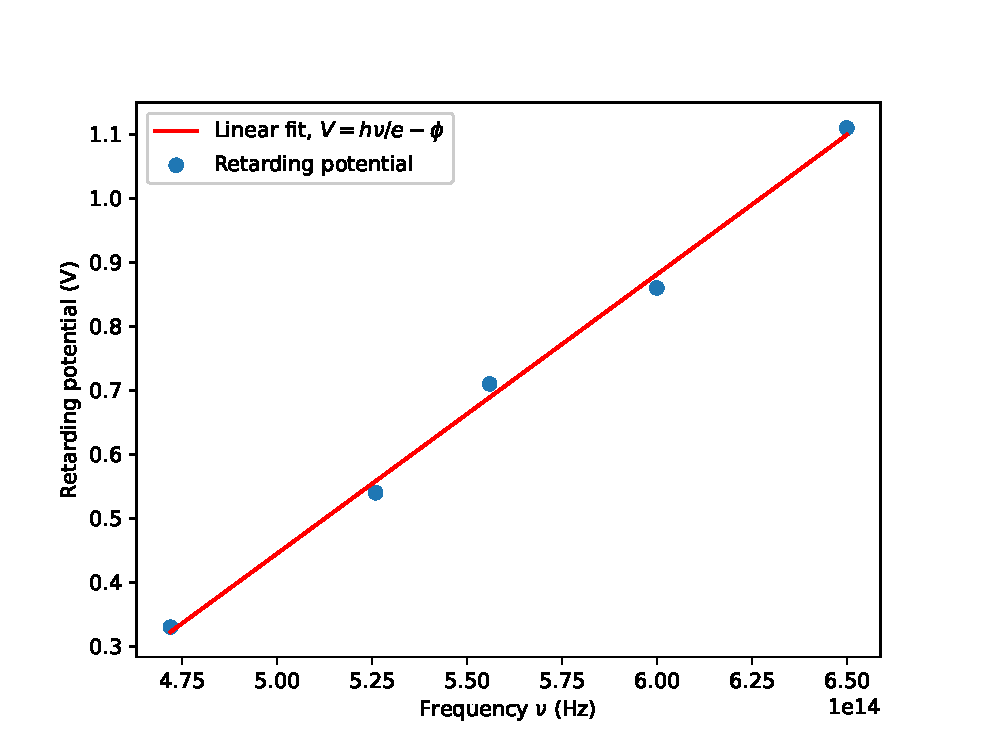
\includegraphics[width=0.7\textwidth]{./planck.eps}
                \caption{Retarding potentials plotted against the frequency of light used and fitted linearly, $V_s = h\nu /q_e - \phi$.}
                \label{fig:planck}
        \end{figure}
        \begin{figure}[H]
                \centering
                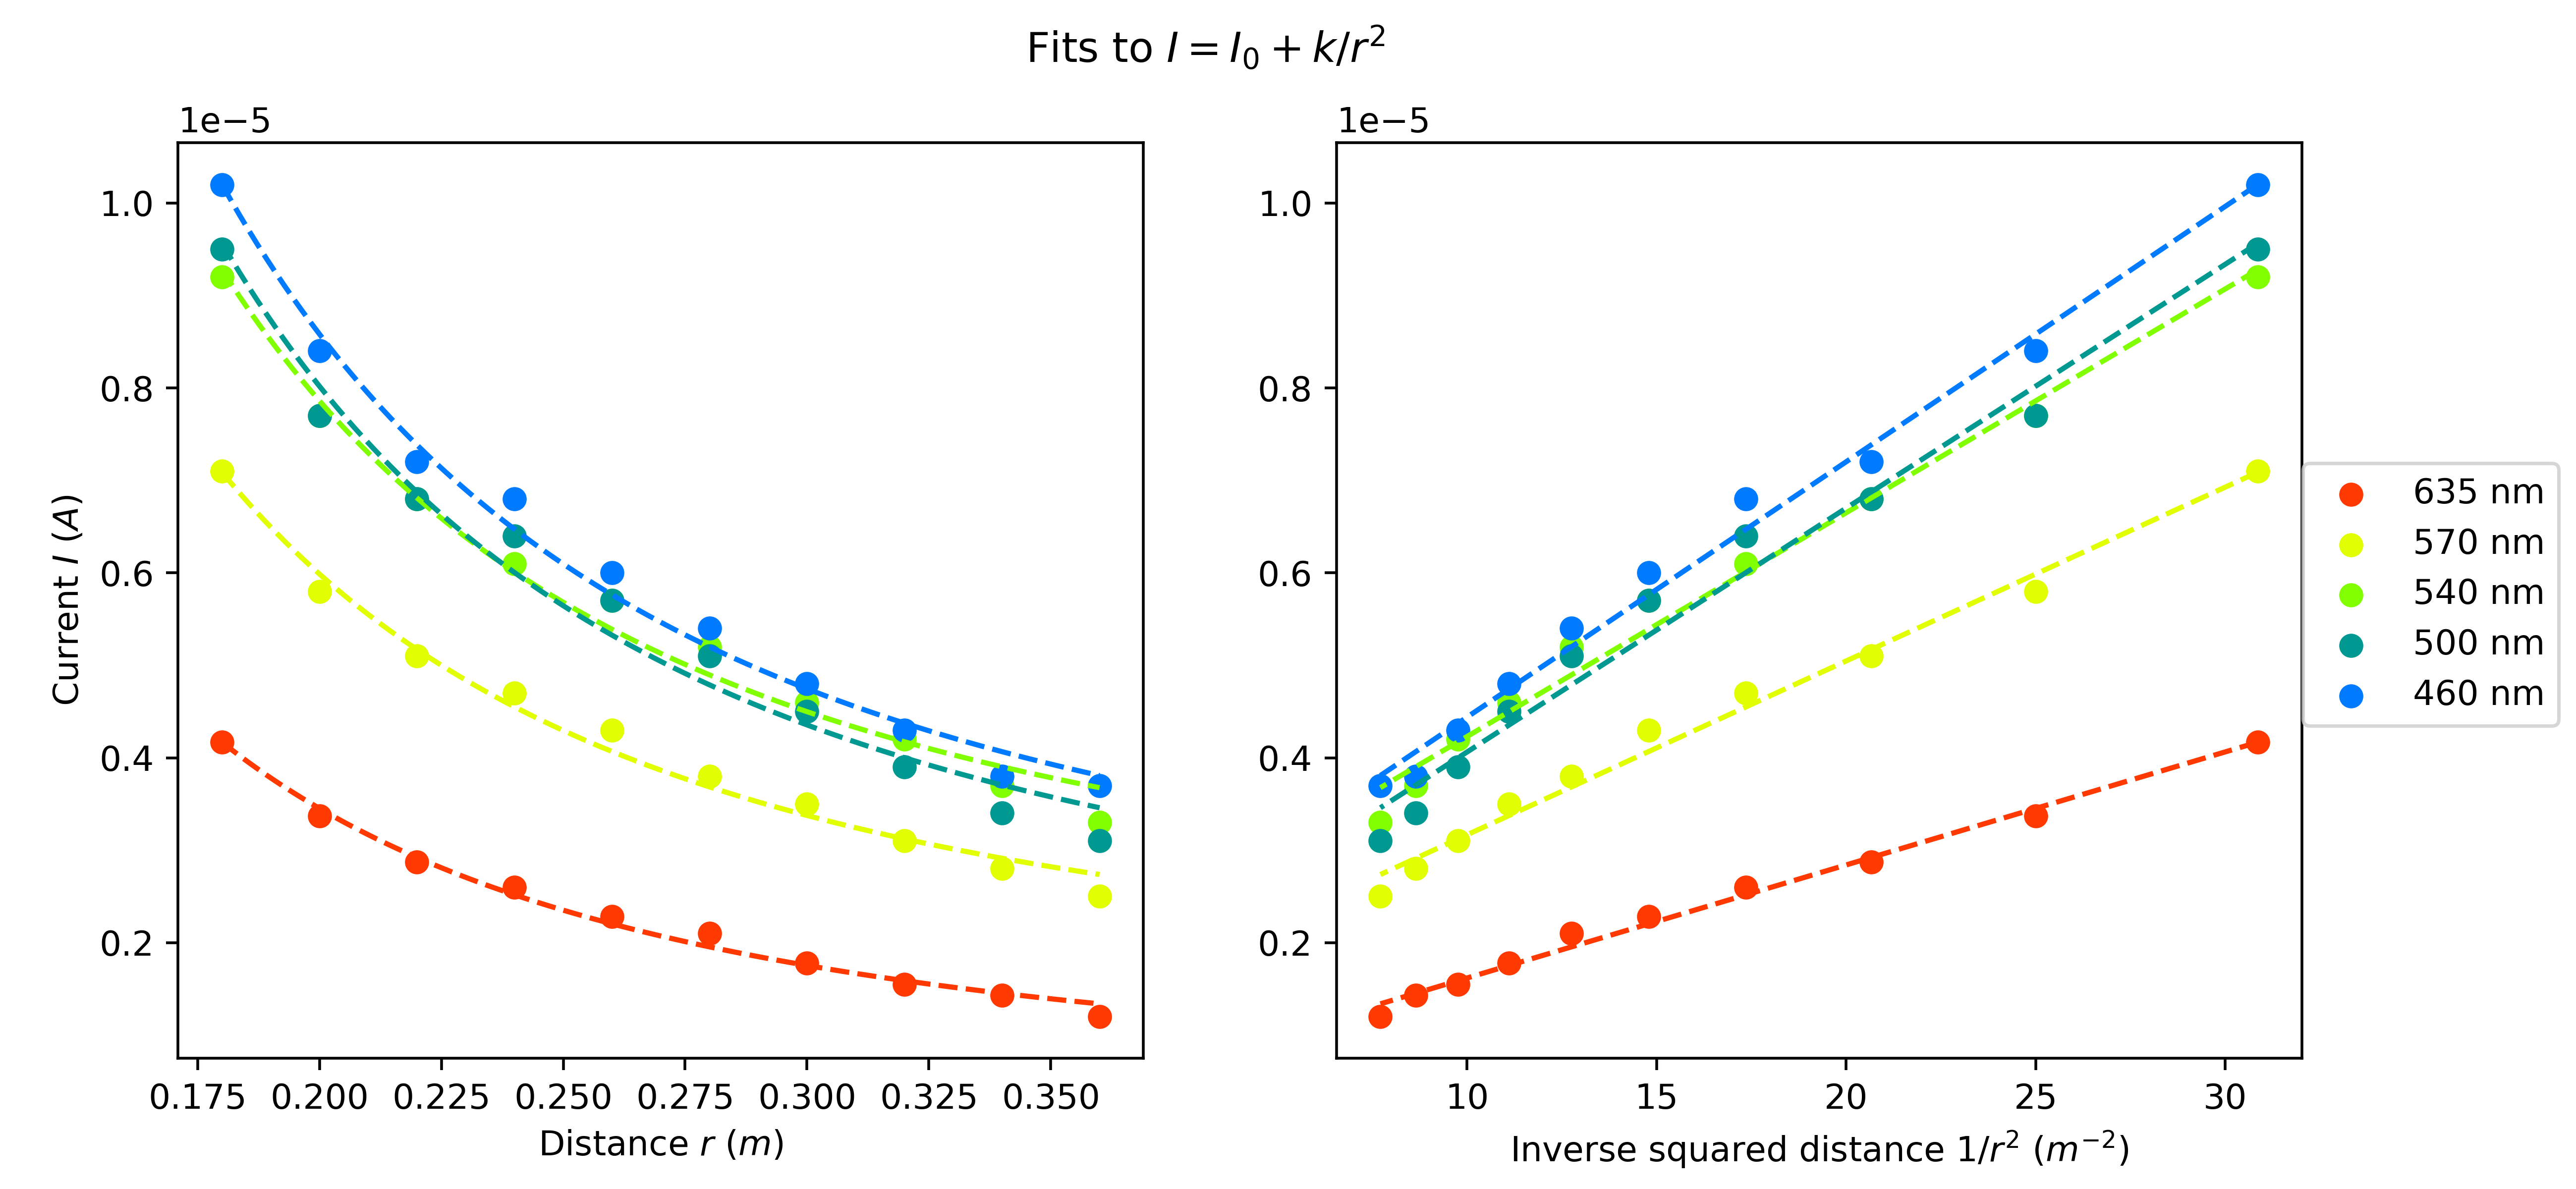
\includegraphics[width=1.1\textwidth]{./inverse.png}
                \caption{Current magnitudes plotted against the distance between the source and the photocell. They obey the inverse square law,
                upto some offset. $V = 0.25$ V.}
                \label{fig:inverse}
        \end{figure}
        From the fit parameters, we have obtained $h = 6.99 \times 10^{-34}$ Js, and $\phi = 1.74$ V.
        The constants $k_\lambda$ are tabulated below.
        \begin{table}[H]
        \caption{Values of $k_\lambda$ and $I_0$ from the fit $I = I_0 + k /r^2$.}
        \centering
        \begin{tabular}{l|ccccc}
                Wavelength $\lambda$ (nm) & 635  & 570  & 540  & 500  & 460  \\
                $k$ ($10^{-7}$ A m$^2$)   & 1.22 & 1.88 & 2.42 & 2.64 & 2.76 \\
                $I_0$ ($10^{-6}$ A)       & 0.39 & 1.29 & 1.81 & 1.42 & 1.68
        \end{tabular}
        \label{tab:slopes}
        \end{table}

        \subsection{Error Analysis}
        The errors in fit parameters are obtained from the covariance matrix of the fit. We see that $\delta h = 0.25 \times 10^{-34}$ Js.
        On the other hand, the deviation from the literature value of Planck's constant ($6.63 \times 10^{-9}$ Js) is
        $0.36 \times 10^{-34}$ Js, which is 5.5\%. This is within $1.5$ standard deviations.

        The error in $\phi$ has been determined as $0.09$ V.
        
        The errors in the slopes $k$ and the currents $I_0$ are tabulated below.
        \begin{table}[H]
        \caption{Uncertainties in $k_\lambda$ and $I_0$ from the fit $I = I_0 + k /r^2$.}
        \centering
        \begin{tabular}{l|ccccc}
                Wavelength $\lambda$ (nm)       & 635  & 570  & 540  & 500  & 460  \\
                $\delta k$ ($10^{-7}$ A m$^2$)  & 0.03 & 0.07 & 0.10 & 0.13 & 0.09 \\
                $\delta I_0$ ($10^{-6}$ A)      & 0.07 & 0.12 & 0.18 & 0.23 & 0.16
        \end{tabular}
        \label{tab:slope_err}
        \end{table}

        \subsection{Reported Values}
        We report $h = (6.99 \pm 0.25) \times 10^{-34}$ Js, which is $5.5$\% higher than the literature value.
        The work function of the metal anode is $W = 1.74 \pm 0.09$ eV.

        \section{Discussion}
        The process of determining Planck's constant is relatively straightforward, and agrees with theory. The error can be attributed to 
        a systematic calibration error in the current measurements.

        We observe that the photocurrent at a fixed voltage fits well with the inverse square law.
        The photocurrent magnitudes are also higher on the blue end, compared to the red end.
        Given that the source or light is a halogen tungsten lamp, we may first suppose that the emitted intensities of different wavelengths
        are unequal, so the photocurrents are naturally unequal. However, such lamps typically have greater intensity towards the red end of the
        spectrum, which is contrary to what we observe.

        Instead, we note that the stopping voltages for the blue light are more negative than for red light, since blue photons
        are more energetic. Only in the limiting case of a very high, positive potential do we observe that the photocurrent for
        light beams of equal intensity and different frequencies become the same, saturated value. In the interim, the current vs
        potential profile is sigmoidal, so the blue curve which starts further back naturally sits above the red curve.
        \begin{figure}[H]
                \centering
                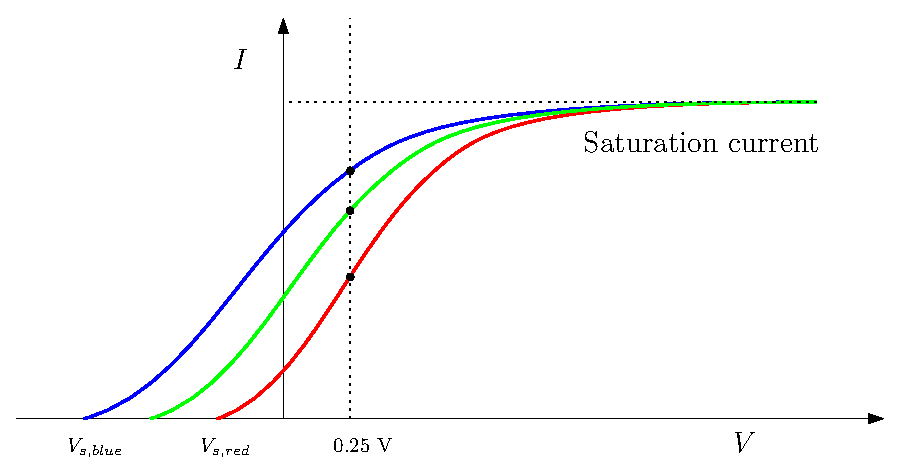
\includegraphics[scale=0.7]{./IV.eps}
                \caption{Photoelectric current vs potential profile, for different frequencies. Note that at a given frequency, the vertical
                line cuts the higher frequencies at higher currents.}
                \label{fig:IV}
        \end{figure}
        

        \subsection{Sources of error}
        Sources of systematic error include incorrect calibrations, extraneous sources of light and buildup of impurities in the photocell.
        The inverse square law fit would suggest that the current readings are slightly shifted, as the $I_0$ parameters are non-zero.
        The filters used may also be imperfect, allowing a band of frequencies to pass through instead of a discrete one.

        \section{Conclusion}
        We thus conclude that light is indeed quantised in terms of energy, and the spread of this energy obeys the inverse square law.

        % \nocite{*}
        % \bibliographystyle{plain}
        % \bibliography{ref}

\end{document}
